Here the problem is the same as the previous step, the only difference is that not only the conversion rates of the customers are unknown, but also the alpha ratios and the number of products sold fo each price.
Since the learners are not able to distinguish the different types of customers, initially the alphas values (probability to start the interaction from a specific product) are uniformly distributed ($[0.2, 0.2, 0.2, 0.2, 0.2]$) and the number of products bought for each price are set all to 1.\\
The same algorithm as before has been developed, with the addictional calculus to estmate the two parametere now uncertain.

\subsection{UCB-1}
The algorithm repeats the same operation as in the previous chapter from step 1 to step 5. Then, it estimate the two parameters:

\begin{itemize}
    \item estimate alpha ratios:\begin{equation}
        \alpha = \alpha + starts
    \end{equation}where starts is a vestor that collects the number of times a customer start from a specific product to visit the web page
    \item estimate number of products sold (version 1):\\
    with this first approach we evaluate this parameters with the empirical mean as can be seen in Equation ~\ref{eqn:num_prod} \begin{equation}
        \label{eqn:mean_items}
        mean\_items[p,a] = \frac{mean\_items[p,a] * seen[p,a] + bought[p]}{estimated\_items[p,a]}
    \end{equation}\begin{equation}
        \label{eqn:num_prod}
        num\_products[p,a] = \frac{1}{mean\_items[p,a]}
    \end{equation}where\begin{itemize}
        \item mean\_items[p,a] in the mean of the number of products {\bf p} with price {\bf a} has been bought till now
        \item seen[p,a] is the number of times products {\bf p} with price {\bf a} has been bought untill the day before
        \item bought[p] is the the total amount of products {\bf p} bought today
        \item estimated\_items[p,a] is the number of times products {\bf p} with price {\bf a} has been bought untill now (so it is seen[p,a] plus the the number of times product p has been bought today)
        \item num\_products[p,a] is the inverse of the value calculated before because represents the parameters of the Geometric distribution, we have used to estimate the number of items bought from the customers, once they have decided to buy that product visualized with that price
    \end{itemize}
    \item estimate number of products sold (version 2):\\
    the calculus of the mean number of products (mean\_items[p,a]) is the same as the other version, so calculated as in Equation ~\ref{eqn:mean_items}. The difference is in the calculus of the parameter of the Geometric distribution, that is done by using a MAB. In this version of the Learner there are two addictional parameters for the mean and the upper bound of this parameters we are trying to estimate. The upper bounds is updated after the Equation ~\ref{eqn:mean_items} and the means when the algorithm want to evaluate which is the best super arm to pull. The results of this version are not shown below, because are much more worst.
\end{itemize}
\subsubsection{Results}
\begin{figure}[ht]
    \begin{center}
    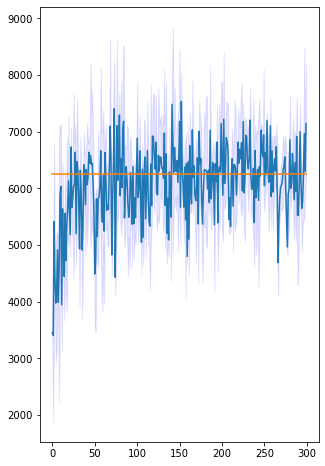
\includegraphics[width=0.6\textwidth]{img/UCB4.png}
    \caption{UCB Reward}
    \label{fig:reward41}
    \end{center}
\end{figure}
\begin{multicols}{2}
    \begin{figure}[H]
        \begin{center}
        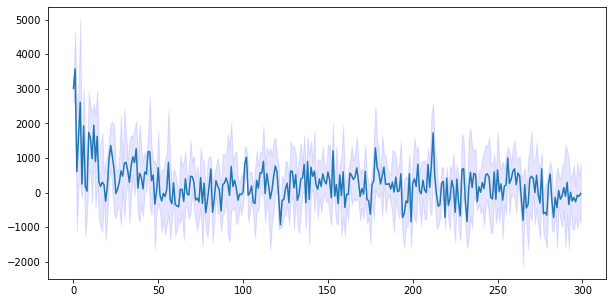
\includegraphics[width=0.5\textwidth]{img/UCB4_regret.png}
        \caption{UCB Regret}
        \label{fig:regret41}
        \end{center}
    \end{figure}
    \columnbreak
    \begin{figure}[H]
        \begin{center}
        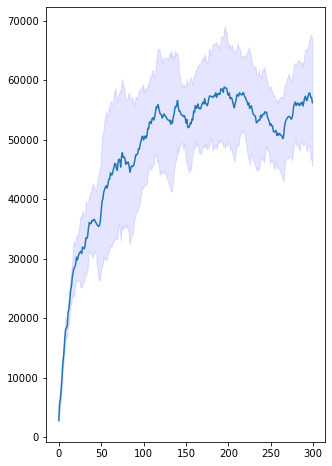
\includegraphics[width=0.5\textwidth]{img/UCB4_cum_reg.png}
        \caption{UCB Cumulative regret}
        \label{fig:cum_reg41}
        \end{center}
    \end{figure}
\end{multicols}

\subsection{TS}
Thomson Sampling 
\begin{figure}[ht]
    \begin{center}
    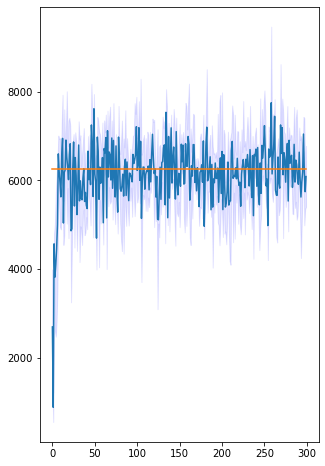
\includegraphics[width=0.6\textwidth]{img/TS4.png}
    \caption{TS Reward}
    \label{fig:reward42}
    \end{center}
\end{figure}
\begin{multicols}{2}
    \begin{figure}[H]
        \begin{center}
        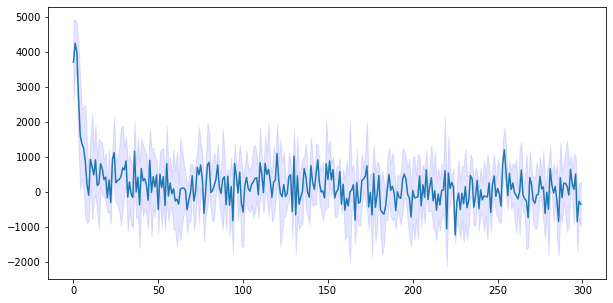
\includegraphics[width=0.5\textwidth]{img/TS4_regret.png}
        \caption{TS Regret}
        \label{fig:regret42}
        \end{center}
    \end{figure}
    \columnbreak
    \begin{figure}[H]
        \begin{center}
        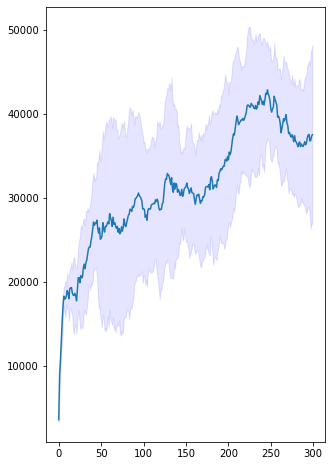
\includegraphics[width=0.5\textwidth]{img/TS4_cum_reg.png}
        \caption{TS Cumulative regret}
        \label{fig:cum_reg42}
        \end{center}
    \end{figure}
\end{multicols}